\documentclass{article}
\usepackage{blindtext}
\usepackage[utf8]{inputenc}
\usepackage{amsmath,bm}
\usepackage{amstext}
\usepackage{amsfonts}
\usepackage{amsmath}
\usepackage{fontspec}
\usepackage{pgfplots}
    \pgfplotsset{compat=1.16}
\usepackage{xeCJK}
    \setCJKmainfont{Songti SC}
    \setCJKsansfont{KaiTi}
\usepackage[colorlinks,linkcolor=blue]{hyperref}
\usepackage{graphicx}
\usepackage{indentfirst}
    \setlength{\parindent}{2em}
\usepackage{listings}
    \lstset { xleftmargin=2em }


\title{Introduction to Machine Learning\\Homework 2}
\begin{document}
    \setlength{\baselineskip}{20pt}
	\maketitle
	\numberwithin{equation}{section}
	\section{[25pts] Multi-Label Logistic Regression}
    \noindent In multi-label problem, each instance $\bm{x}$ has a label set $\bm{y}=\{y_1,y_2,...,y_l\}$ and each label $y_i\in\{0,1\}$. Assume the post probability $p(\bm{y}|x)$ follows the conditional independence:\\
    \begin{equation}
    p(\bm{y}|x)=\prod\limits_{i=1}^l p(y_i|x).
    \end{equation}
    Please use the logistic regression method to handle the following questions.\\
    (1) [15pts] Please give the 'log-likelihood' function of your logistic regression model;\\
    (2) [10pts] Please calculate the gradient of your 'log-likelihood' function.\\ \\
    (1) 由题意可知,各个标签对应的事件是条件独立的。所以可将此多标签逻辑回归模型(并行地)分解为 $l$ 个二分类的逻辑回归模型。\\
        设 $B = \begin{pmatrix} \beta_1 & \beta_2 & \cdots & \beta_l \end{pmatrix}$,其中 $\beta_{i} = (w_i;b_i)$,同时设 $\hat{x} = (x;1)$,故 $\hat{y} = B^T \hat{x}$,再令 $p_1(\hat{x};\beta_{j}) = p(y=1\mid\hat{x};\beta_{j}) = \frac{1}{1 + \mathrm{e}^{-\beta_j^T \hat{x}}}$,$p_0(\hat{x};\beta_{j}) = p(y=0\mid\hat{x};\beta_{j}) = 1-p_1(\hat{x};\beta_{j})$,可知 $p_1(\hat{x};B) = \left(p_1(\hat{x};\beta_1), p_1(\hat{x};\beta_2), \cdots, p_1(\hat{x};\beta_l)\right)$,$p_0(\hat{x};B) = \left(p_0(\hat{x};\beta_1), p_0(\hat{x};\beta_2), \cdots, p_0(\hat{x};\beta_l)\right)$,因此该逻辑回归模型的“对数似然”函数为:\\
        \begin{equation}
        \begin{aligned}
        \ell(B)
        &= \sum_{i=1}^{m} \ln p(y_i\mid \hat{x_i};B) \\
        &= \sum_{i=1}^{m} y_i\ln p_1(\hat{x_i};\beta_{j}) + (1-y_i)\ln p_0(\hat{x_i};\beta_{j}) \\
        &= \sum_{i=1}^{m} y_i\ln\frac{1}{1+\mathrm{e}^{-B^{T}\hat{x_i}}} + (1-y_i)\ln \left(1-\frac{1}{1+\mathrm{e}^{-B^{T}\hat{x_i}}}\right)\\
        \end{aligned}
        \end{equation} \\
    (2) 设 $g(z) = \frac{1}{1+\mathrm{e}^{-z}}$,易知其导数 $g'(z) = g(z)\left(1-g(z)\right)$,因此 $\ell(B)$ 的梯度为:\\
        \begin{equation}
        \begin{aligned}
        \frac{\partial\ell(B)}{\partial B}
        &= \sum_{i=1}^{m} \left(y_i\frac{1}{g(B^T\hat{x_i})}-(1-y_i)\frac{1}{1-g(B^T\hat{x_i})}\right) \frac{\partial g(B^T\hat{x_i})}{\partial B} \\
        &= \sum_{i=1}^{m} \left(y_i\frac{1}{g(B^T\hat{x_i})}-(1-y_i)\frac{1}{1-g(B^T\hat{x_i})}\right) g(B^T\hat{x_i}) (1-g(B^T\hat{x_i})) \frac{\partial(B^T\hat{x_i})}{\partial B} \\
        &= \sum_{i=1}^{m} \left(y_i(1-g(B^T\hat{x_i}))-(1-y_i)g(B^T\hat{x_i})\right) \hat{x_i} \\
        &= \sum_{i=1}^{m} \left(y_i-g(B^T\hat{x_i})\right) \hat{x_i} \\
        &= \sum_{i=1}^{m} \left(y_i-\frac{1}{1+\mathrm{e}^{-B^T\hat{x_i}}}\right) \hat{x_i}
        \end{aligned}
        \end{equation}


\vspace{3cm}


	\numberwithin{equation}{section}
	\section{[20pts] Linear Discriminant Analysis}
	
	\noindent Suppose we transform the original $\bf X$ to $\hat{\bf Y}$ via linear regression. In detail, let 
	
	\begin{equation*}
	\hat{\bf Y} = \bf X(\bf X^{\top} \bf X)^{-1}\bf X^{\top}\bf Y = \bf X\hat{\bf B},
	\end{equation*}
	where $\bf X$ and $\bf Y$ are the feature and label matrix, respectively.
	 Similarly for any input $\mathbf{x}$, we get a transformed vector $\hat{\mathbf{y}} = \hat{\bf B}^{\top}\mathbf{x}$. Show that LDA using $\hat{\bf Y}$ is identical to LDA in the original space. \\ \\
    设 $\bf X_j\ (j=1,2,\cdots,k)$ 为第 $j$ 类样本的集合(总共有 $k$ 类),即 $\bf X = \bf X_1 \cup \bf X_2 \cup \cdots \cup \bf X_k$,$m_j$ 为第 $j$ 类样本的个数。\\
    定义 $\mu_j$、$\mu_{jy}$ 和 $\Sigma_j$、$\Sigma_{jy}$ 分别为第 $j$ 类样本及其线性变换后样本($\bf \hat{Y}$)的均值向量和协方差矩阵。则有:\\
    \begin{align}
    \mu_{jy} &= \frac{1}{m_j}\sum_{\hat{y}\in \hat{Y}_j}\hat{y} = \frac{1}{m_j}\sum_{x\in X_j}\hat{B}^T x = \hat{B}^T \mu_j \\
    \Sigma_{jy}
    &= \sum_{\hat{y}\in \hat{Y}_j} (\hat{y} - \mu_{jy}) (\hat{y} - \mu_{jy})^T \quad \text{// 忽略分母常数} \\
    &= \sum_{x\in X_j} (\hat{B}^T x-\hat{B}^T \mu_j) (\hat{B}^T x-\hat{B}^T \mu_j)^T \\
    &= \hat{B}^T \Sigma_j \hat{B} \\
    \end{align}
    设 $\bf Y_j$ 为第 $j$ 类样本的标签(即 $\bf Y$ 的第 $j$ 列),则有:
    \begin{equation}
    \mu_j = \frac{1}{m_j}\sum_{x\in X_j}x = \frac{1}{m_j} X^T Y_k \\
    \end{equation}
    以全部样本的角度看,设 $D = \mathrm{diag}(\frac{1}{m_1}, \frac{1}{m_2}, \cdots, \frac{1}{m_k})$,有:\\
    \begin{align}
    \mu &= X^T YD \\
    \Sigma
    &= (X^T - X^T YDY^T) (X^T - X^T YDY^T)^T \\
    &= X^T (I - YDY^T)^2 X \\
    &= X^T (I - YDY^T) X \\
    \end{align}
    同时,$\Sigma_y = \hat{B}^T \Sigma \hat{B}$\\
    由于 LDA 拥有线性判别边界,且其边界决定于判别函数\cite{ref1},即:
    \begin{equation}
    \delta_j(x) = \log\pi_j - \frac{1}{2}\mu_j^T\Sigma^{-1}\mu_j + x^T\Sigma^{-1}\mu_j \\
    \end{equation}
    对于 $\hat{Y}$,其判别函数为:
    \begin{equation}
    \delta_j = \log\pi_j - \frac{1}{2}\mu_{jy}^T\Sigma_y^{-1}\mu_{jy} + \hat{Y}\Sigma_y^{-1}\mu_{jy} \\
    \end{equation}
    接下来只要证明用 $\bf \hat{Y}$ 表示的判别函数和用 $\bf X$ 表示的等价,即可证明对应的 LDA 等价。\\
    (1) 对于 $\log\pi_j$,显然其概率已经在数据集中确定,不会受到 $\bf X$ 变换的影响,故在两个判别函数中是相等的。\\
    (2) 对于 $\hat{Y}\Sigma_y^{-1}\mu_{jy}$,将其展开可得:
    \begin{equation}
    \hat{Y}\Sigma_y^{-1}\mu_{jy} = (X\hat{B}) (\hat{B}^T \Sigma \hat{B})^{-1} (\frac{1}{m_j}\hat{B}^T X^T Y_k)
    \end{equation}
    以全部样本的角度看,则上式转化为:
    \begin{equation}
    \hat{Y}\Sigma_y^{-1}\mu_{y} = (X\hat{B}) (\hat{B}^T \Sigma \hat{B})^{-1} (\hat{B}^T X^T YD)
    \end{equation}
    对 $\hat{B}^T \Sigma \hat{B}$ 展开:
    \begin{equation}
    \begin{aligned}
    \hat{B}^T \Sigma \hat{B}
    &= \hat{B}^T X^T (I - YDY^T) X \hat{B} \\
    &= \hat{B}^T X^T X\hat{B} - \hat{B}^T X^T YDY^T X\hat{B} \\
    &= Y^T X (X^T X)^{-1} X^T X (X^T X)^{-1} X^T Y - \hat{B}^T X^T YDY^T X\hat{B} \quad\text{// $((X^T X)^{-1})^T = (X^T X)^{-1}$} \\
    &= \hat{B}^T X^T Y - \hat{B}^T X^T YDY^T X\hat{B} \\
    &= Y^T Y - Y^T Y D Y^T Y \\
    \end{aligned}
    \end{equation}
    设 $P = Y^T Y$,则 $\hat{B}^T \Sigma \hat{B} = P - PDP = P(I - DP)$,继续展开式子(2.15):\\
    \begin{equation}
    \begin{aligned}
    \hat{Y}\Sigma_y^{-1}\mu_{y} 
    &= (X\hat{B}) (\hat{B}^T \Sigma \hat{B})^{-1} (\hat{B}^T X^T YD) \\
    &= X\hat{B}(P(I-DP))^{-1}\hat{B}^T X^T YD \\
    &= X\hat{B}(I-DP)^{-1}P^{-1}PD \\
    &= X\Sigma^{-1}\Sigma\hat{B}(I-DP)^{-1}D \\
    &= X\Sigma^{-1}X^T (I-YDY^T) X\hat{B}(I-DP)^{-1}D \\
    &= X\Sigma^{-1}(X^T X\hat{B} - X^T YDY^T X\hat{B})(I-DP)^{-1}D \\
    &= X\Sigma^{-1}(X^T Y - X^T YDP)(I-DP)^{-1}D \\
    &= X\Sigma^{-1}X^T Y(I-DP)(I-DP)^{-1}D \\
    &= X\Sigma^{-1}X^T Y D \\
    &= X\Sigma^{-1}\mu \\
    \end{aligned}
    \end{equation} 
    故可得该部分与 $\bf X$ 的判别函数对应部分等价。 \\
    (3) 对于 $\frac{1}{2}\mu_{jy}^T\Sigma_y^{-1}\mu_{jy}$,从全局角度看,将后面的 $\mu_{jy}$ 表示为 $\mu_y$,可得:
    \begin{equation}
    \begin{aligned}
    \frac{1}{2}\mu_{jy}^T\Sigma_y^{-1}\mu_y
    &= (\hat{B}^T \mu_j)^T\Sigma_y^{-1}(\hat{B}^T X^T YD) \\
    &= \mu_j^T\hat{B}\Sigma_y^{-1}(\hat{B}^T X^T YD) \\
    &= \mu_j^T\hat{B}(\hat{B}^T\Sigma\hat{B})^{-1}\hat{B}^T X^T YD \\
    &= \mu_j^T\Sigma^{-1}X^T Y D \quad\text{// 由式子(2.17)过程可得$\hat{B}(\hat{B}^T\Sigma\hat{B})^{-1}\hat{B}^T = \Sigma^{-1}$}\\
    &= \mu_j^T\Sigma^{-1}\mu
    \end{aligned}
    \end{equation}
    同样该部分与 $\bf X$ 的判别函数对应部分等价。\\
    综上可知在 $\bf \hat{Y}$ 上做线性判别分析与在 $\bf X$ 上做是相同的。

    \begin{thebibliography}{10}
    \bibitem{ref1} Stanford STATS 202. https://web.stanford.edu/class/stats202/content/lec9.pdf
    \end{thebibliography}
    
\vspace{3cm}


\numberwithin{equation}{section}
\section{[55pts] Logistic Regression from scratch  }
\noindent Implementing algorithms is a good way of understanding how they work in-depth. In case that you are not familiar with the pipeline of building a machine learning model, this article can be an example (\href{https://www.jianshu.com/p/ecb89148ed64}{here}).

In this experiment, you are asked to build a classification model on one of UCI data sets, Letter Recognition Data Set
(\href{http://lamda.nju.edu.cn/ml2019/ML2019-PS2-dataset.zip}{click to download}). In particular, the objective is to identify each of a large number of black-and-white
rectangular pixel displays as one of the 26 capital letters in the English alphabet. The detailed statistics of this data set is listed in Table~\ref{tab:dataset}. The data set was then randomly split into train set and test set with proportion $7:3$. Also, letters from `A' to `Z' are mapped to digits `1' to `26' respectively as represented in the last column of the provided data set.


\begin{table}[!ht]
    \centering
    \caption{Statistics of the data set.}
    \vspace{2mm}
    \label{tab:dataset}
    \begin{tabular}{|c|c|c|}
    \hline
    Property & Value & Description\\
    \hline
        Number of Instances & 20,000 & Rows of the data set\\
    \hline
        Number of Features & 17 & Columns of the data set\\
    \hline
        Number of classes & 26 & Dimension of the target attribute \\
    \hline
    \end{tabular}
\end{table}


In order to build machine learning models, you are supposed to implement Logistic Regression (LR) algorithm which is commonly used in classification tasks. Specifically, in this experiment, you have to adapt the traditional binary class LR method to tackle the multi-class learning problem. 

\begin{enumerate}
    \item[(1)] [\textbf{5pts}] You are encouraged to implement the code using \emph{Python3} or \emph{Matlab}, implementations in any other programming language will not be judged. Please name the source file (which contains the main function) as \emph{LR\underline{\hspace{0.5em}}main.py} (for python3) or \emph{LR\underline{\hspace{0.5em}}main.m} (for matlab). Finally, your code needs to print the testing performance on the provided test set once executed.

    \item[(2)] [\textbf{30pts}] Functions required to implement:
    \begin{itemize}
        \item Implement LR algorithm using gradient descent or Newton's method.
        \item Incorporate One-vs-Rest (OvR) strategy to tackle multi-class classification problem.
    \end{itemize}
    \item[(3)] [\textbf{20pts}] Explain implementing details in your submitted report (source code should not be included in your report), including optimization details and hyper-parameter settings, etc. Also, testing performance with respect to Accuracy, Precision, Recall, and $F_1$ score should be reported following the form of Table 2.
\end{enumerate}

\begin{table}[h]
    \centering
     \caption{Performance of your implementation on test set.}
     \vspace{2mm}
    \label{tab:my_label}
    \begin{tabular}{|c|c|}
       \hline
       Performance Metric & Value (\%) \\
       \hline
       accuracy & 00.00 \\
       \hline
       micro Precision  & 00.00\\
       \hline
       micro Recall & 00.00\\
       \hline
       micro $F_1$ & 00.00\\
       \hline
       macro Precision  & 00.00\\
       \hline
       macro Recall & 00.00\\
       \hline
       macro $F_1$ & 00.00\\
       \hline
    \end{tabular}

\end{table}

\textbf{NOTE:} Any off-the-shelf implementations of LR or optimization methods are \textbf{NOT ALLOWED} to use. When submitting your code and report, all files should be placed in the same directory (without any sub-directory).

\clearpage
\noindent\textbf{实验报告.}
\subsection{实验目的与简介}
本次实验使用UCI数据集和多分类逻辑回归模型处理多分类问题,目的是通过基于多类别的逻辑回归方法,学习数据集中图像表示的字母与其图像特征的关系,使分类器能够在接收新的图片特征时对其表示的字母进行较准确的预测。同时,通过这项实验,能够体会到机器学习任务的基本流程。\\
\indent 本次实验使用 Python3 编程语言进行实现,以下是基本流程图。\\
\indent 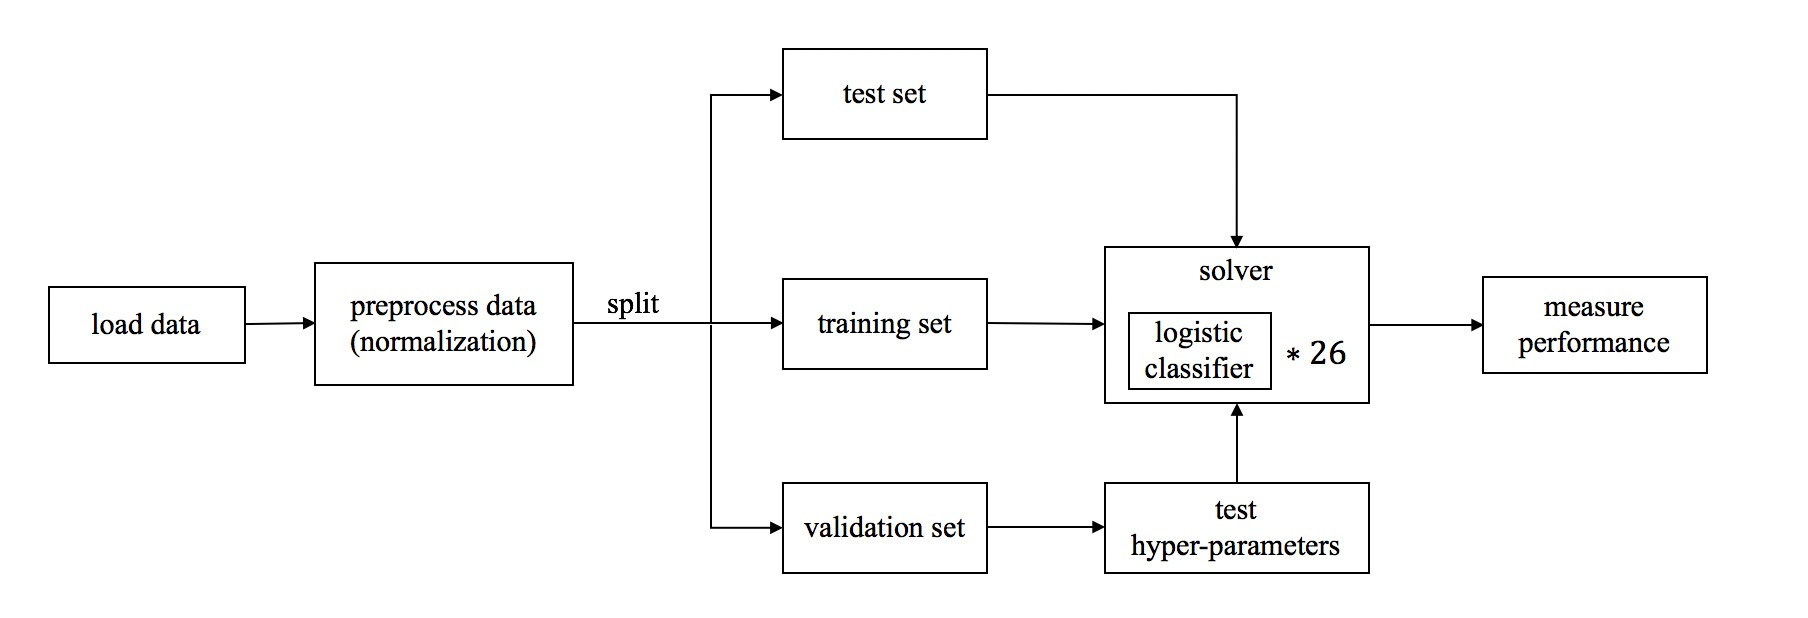
\includegraphics[width = 0.9\textwidth]{flow-chart.jpg} \\

\subsection{数据加载及预处理}
本次实验的原始数据集文件格式有 txt、csv 两种,故可以使用pandas数据处理包对 csv 文件进行方便的读取、拆分和转化成 numpy 数组。同时,将训练数据集以 9:1 的比例拆分成训练集和验证集。(最终不用 k-fold 验证的原因是实验采用 OvR 的方式处理多分类问题,需要同时训练 26 个二分类器,耗时较多,并且采用过十折交叉验证,效果与普通验证方案差别并不大)\\
\indent 经过简单的检查,原始数据集中并没有数据缺失、不合格的情况,无需进行额外的数据清洗、填补工作。
\subsubsection{数据标准化}
\indent 在逻辑回归模型中,输入数据的每个特征与其权重直接相乘,故数据特征的规模(数量级)对参数调整的影响很大,因此有必要对数据的各个特征进行标准化。\\
\indent 标准化方法是每个特征值减去该特征在数据集中的均值并除以该特征的标准差。同时,这一过程在训练集中进行,验证集及测试机直接采用训练集各特征的均值和标准差进行标准化,以保证数据对噪声有较好的忍受度。\\
\indent 实验也会比较数据标准化与否与模型预测性能的影响。

\subsection{构建多分类算法}
\indent 本实验需要解决一个识别 A-Z 的 26 分类问题,采用 OvR 的策略来实施,因此需要分别训练 26 个分类器:$C_{1}, C_{2}, \cdots, C_{26}$。每个分类器 $C_i$ 以第 $i$ 个字母为正例,其余字母为负例进行训练。\\
\indent 在代码实现中,我将逻辑回归模型抽象成一个类 LogisticClassifier,用 Solver 类对其进行参数设置、训练和测试。
\subsubsection{单个分类器构建,以$C_1$为例}
\indent 在对单个分类器进行数据传入时,首先要要将数据标签 $y$ 进行预处理,即将第一个标签 1 标记为正例(1),其余标记为负例(0)。同时,将标准化后的数据 X 加上一列常数向量 $(1, 1, \cdots,  1)^T$,并令 $\beta = (W;b)$ 以简化模型。\\
\indent 分类器的优化算法为梯度下降法,其中 loss 和 grad 的计算定义在方法 LogisticClassifier.loss() 中。
\subsubsection{类别不均衡问题}
\indent 对于类别不均衡问题,采用阈值移动的方法,经过测试,将阈值设置为 0.3。

\subsubsection{整合分类结果}
\indent 在 Solver 中用测试集/验证集同时对 26 个分类器进行测试并各自得出结果,每个分类器得出 m 个分数(假设输入实例个数为 m),再对各个模型的分数进行比较,取出分数最高的分类器对应的标签作为分类结果。

\subsection{超参数分析}
\indent 在实验中,我主要设置了以下几个超参数,以验证集准确率为性能指标。在对某个超参数进行比较时,取其他超参数取得最好验证性能的值作为基础。
\subsubsection{是否标准化}
\begin{table}[!htbp]
    \begin{tabular}{|l|l|l|}
    \hline
    normalization?                                                       & Yes & No  \\ \hline
    \begin{tabular}[c]{@{}l@{}}accuracy of\\ validation set\end{tabular} & 0.722143 & 0.662143 \\ \hline
    \end{tabular}
\end{table}
\subsubsection{学习率}
\begin{table}[!htbp]
    \begin{tabular}{|l|l|l|l|}
    \hline
    learning rate                                                        & 0.00001 & 0.001 & 0.01 \\ \hline
    \begin{tabular}[c]{@{}l@{}}accuracy of\\ validation set\end{tabular} & 0.477857 & 0.691429 & 0.722143  \\ \hline
    \end{tabular}
\end{table}
\subsubsection{正则化参数}
\begin{table}[!htbp]
    \begin{tabular}{|l|l|l|l|}
    \hline
    \begin{tabular}[c]{@{}l@{}}regularization\\ strength\end{tabular}    & 0   & 0.00001 & 0.001 \\ \hline
    \begin{tabular}[c]{@{}l@{}}accuracy of\\ validation set\end{tabular} & 0.722143 & 0.720000 & 0.712143   \\ \hline
    \end{tabular}
\end{table}
\subsubsection{迭代次数}
\begin{table}[!htbp]
    \begin{tabular}{|l|l|l|l|l|}
    \hline
    num of epoch                                                         & 10  & 30  & 70  & 100 \\ \hline
    \begin{tabular}[c]{@{}l@{}}accuracy of\\ validation set\end{tabular} & 0.694286 & 0.710714 & 0.719286 & 0.722143 \\ \hline
    \end{tabular}
\end{table}
\subsubsection{batch 大小}
\begin{table}[!htbp]
    \begin{tabular}{|l|l|l|l|}
    \hline
    batch size                                                           & 10  & 50  & 100 \\ \hline
    \begin{tabular}[c]{@{}l@{}}accuracy of\\ validation set\end{tabular} & 0.722143 & 0.709286 & 0.690714 \\ \hline
    \end{tabular}
\end{table}
\quad \\
从以上数据可知,最佳超参数组合为:
\begin{lstlisting}
    normalize = True
    learning_rate = 0.0
    regularization_strength = 0.001
    num_epochs = 100
    batch_size = 10
\end{lstlisting}
其中值得注意的是正则化参数越高,验证集准确率反而偏低。推测是在正则化时分类器参数 W 的值会趋向于整体变小,通过 Sigmoid 函数后正负类的分数不能明显拉开,导致在比较时各个分类器分数时误差较大。

\subsection{一些尝试}
\subsubsection{动量方法}
在优化方法中,我在梯度下降法的基础上使用动量方法,以求加快模型的收敛速度和尽可能提高精确度,但经过测试之后准确度反而降低了大约 10\%。
\subsubsection{权重的初始化}
在逻辑回归分类器的初始化中,我尝试了参数值 —— 权重 W 不同规模的初始化,其初始化代码为:
\begin{lstlisting}
W = np.random.normal(0, weight_scale, (input_dim,))
\end{lstlisting}
\indent 我将 $weight\_scale$ 设置为 $1e^{-5},\; 1e^{-3},\; 1$ 三个不同的值,但验证集测试的结果差别不大,最终设置 $weight\_scale = 1e^{-3}$。

\subsection{测试集表现}
最终测试性能如表3所示:
\begin{table}[!htbp]
    \centering
     \caption{Performance of your implementation on test set.}
     \vspace{2mm}
    \label{tab:my_label}
    \begin{tabular}{|c|c|}
       \hline
       Performance Metric & Value (\%) \\
       \hline
       accuracy & 72.42 \\
       \hline
       micro Precision  & 64.38 \\
       \hline
       micro Recall & 56.52 \\
       \hline
       micro $F_1$ & 60.19 \\
       \hline
       macro Precision  & 60.04 \\
       \hline
       macro Recall & 56.54 \\
       \hline
       macro $F_1$ & 58.24 \\
       \hline
    \end{tabular}
\end{table}

\subsection{复现结果}
执行以下语句,会以最佳参数执进行训练过程,并显示最终测试准确度。
\begin{lstlisting}
python3 LR_main.py
\end{lstlisting}

\end{document}